\emph{
	Haga un programa en octave que permita simular las trayectorias de una 
	cadena de Markov a tiempo continuo $X$ con matriz infinitesimal $Q$.\pn
}

\afterstatement\pn

Para poder reutilizar el código en el siguiente inciso, esta parte se
programó como una función de \texttt{Tmax}. \texttt{Tmax} que representa una cota para el tiempo
que se representa en la ejecución de la Cadena de Markov.\pn

\small
\texttt{
	\lstinputlisting[inputencoding=utf8]{tarea5/problema5_8/SimMarkov.m}
}
\normalsize

A continuación una imagen que resultó de ejecutar esta función

\begin{center}
    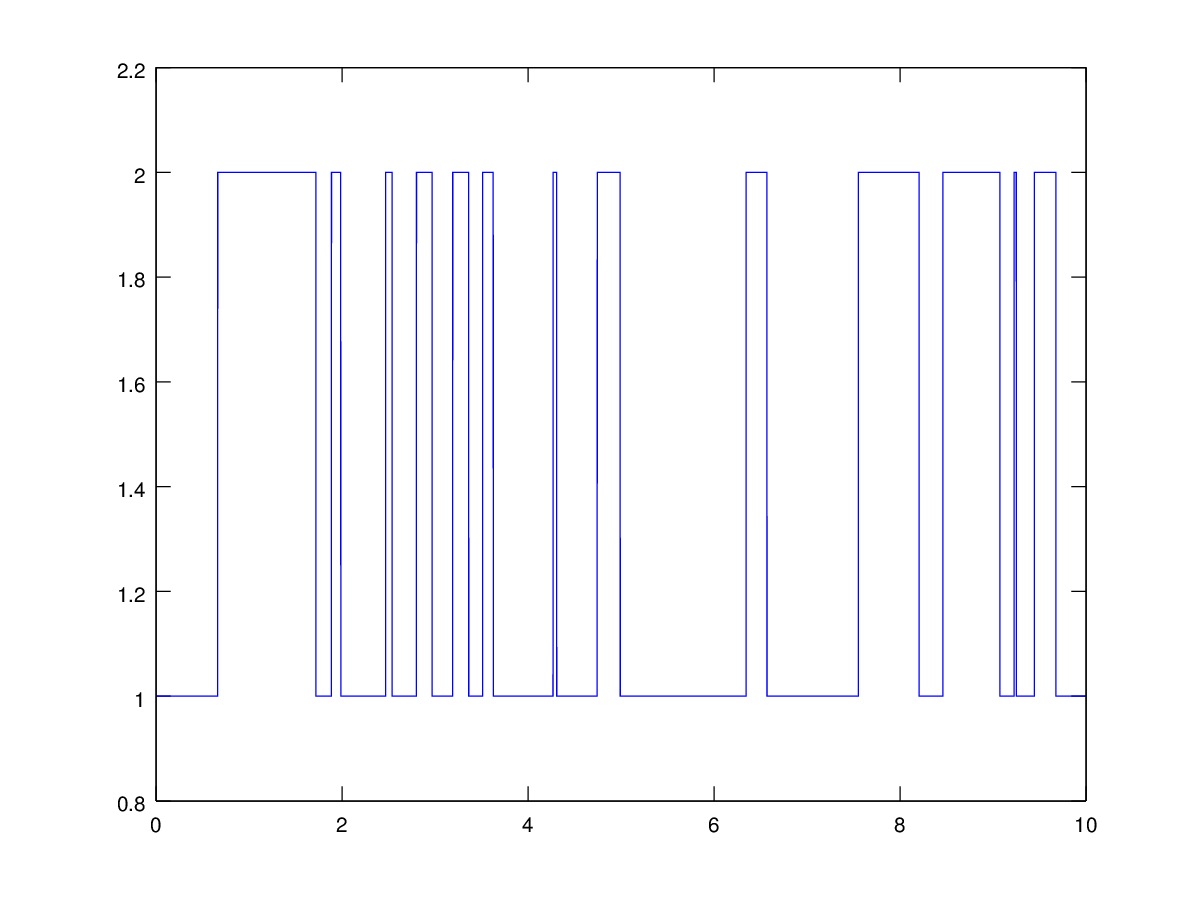
\includegraphics[width=8cm]{tarea5/problema5_8/MarkovHasta10.png}
\end{center}